
\documentclass[journal]{IEEEtran}
\usepackage{xeCJK}


\ifCLASSINFOpdf

\else

\fi

\hyphenation{op-tical net-works semi-conduc-tor}

% 添加reference 依赖的包
\usepackage[utf8]{inputenc}
\usepackage{graphicx} % 图像显示
\usepackage[justification=centering]{caption} %caption居中
\usepackage[sorting=none]{biblatex}
\usepackage{booktabs} % 表格

\usepackage{fontspec} % 字体

\usepackage{float}  %引入float宏包
\usepackage{bm} % 加黑


\addbibresource{reference.bib}
% 图片依赖的路径
\graphicspath{{chapter and images}}

\begin{document}
% 标题
\title{MLSA-YOLOV8: an efficient infrared remote sensing small object detection based on label assignment strategy and tiny head}
% 作者信息
\author{Yi~Li, Huajun~Wang}

\markboth{}% 标签
{Shell \MakeLowercase{\textit{et al.}}: Bare Demo of IEEEtran.cls for Journals}

\maketitle

%摘要
\begin{abstract}
aa
\end{abstract}

% 关键字
\begin{IEEEkeywords}
Infrared small object detection, Label Assignment, Prediction Head, Anchor Free
\end{IEEEkeywords}

\IEEEpeerreviewmaketitle

% Introduction
\section{Introduction}

\IEEEPARstart{I}{nfrared} imaging systems can detect objects at any time of day, making them a significant technological advancement. Their capacity to capture heat sources further enhances their functionality, providing a comprehensive view of the environment. Coupled with their extensive range, these systems offer unparalleled surveillance capabilities. These features make them critical optoelectronic components in surveillance systems\cite{dai2023one}. Robust small object detection is important to infrared search and tracking applications. Moreover, it has been an investigatory hot spot \cite{zhao2022single}. Generic object detectors are categorized into: anchor-based and anchor-free patterns. However, their performance on small-target tasks suffers from unreasonable label assignment of small targets and low resolution after CNN drop sampling
\cite{xu2022rfla}.

% 标签分配

\subsection{Label Assignment Strategy}
Location, as one of the main tasks of detection, is expressed as a regression problem in most detection paradigms, where the location branch is designed as an output boundary box offset, and the joint intersection (lou) metric is usually used to evaluate the accuracy\cite{zhu2021tph}. FasterRCNN and RetinaNet select the IoU threshold of pre-defined anchors and ground truth to distinguish positive and negative samples \cite{ren2015faster}\cite{lin2017focal}. Considering the distance between center points, overlapping parts, along with aspect ratio. yolov4 chose CIoU as the label Assignment Tactic can fulfill greater convergence velocity and precision on the BBox regression \cite{bochkovskiy2020yolov4}.  FCOS chooses anchors located in the central region of ground truth as its positive sample\cite{tian2019fcos}. The IoU metric, however, exhibits a significant bias towards larger objects and demonstrates high sensitivity to small infrared targets owing to their diminutive size . As shown in the\ref{fig: IOU}, small deviations (6 pixels along diagonal orientation) in small object prediction box caused a significant drop in loU (from 72$\%$ to 38$\%$) compared to normal objects (96$\%$ and 92$\%$). In other words, Compared with regular objects IoU is vulnerable to light offset between two boundary boxes, and this ambiguous anchors assignment can affect the learning of regression branches\cite{xu2021dot}. We call this problem Low tolerance for bounding box perturbation \cite{zhao2022single}.  Given the above problems,  Xu put forward dot distance, they think very small objects could be regarded as points and the importance of height and breadth is far lower than that of the locations of center points. Hence, DotD centers uniquely on the positional correlation between center points, and the correlation becomes more appropriate for tiny targets of absolute size below 16 pixels\cite{xu2021dot}. However, the dot method needs to calculate each pixel point. When the target is too large, the computational complexity is high. To tackle the performance difference in infrared tiny object detection, a new label assignment plan is brought forward, which is known as the Multi-scale label assignment strategy. We continue to utilize CIOU as the label allocation index for low-resolution large maps and reference DotD for high-resolution feature maps in order to further enhance the detection rate of minimal targets.

\begin{figure}[!t]
    \centering
    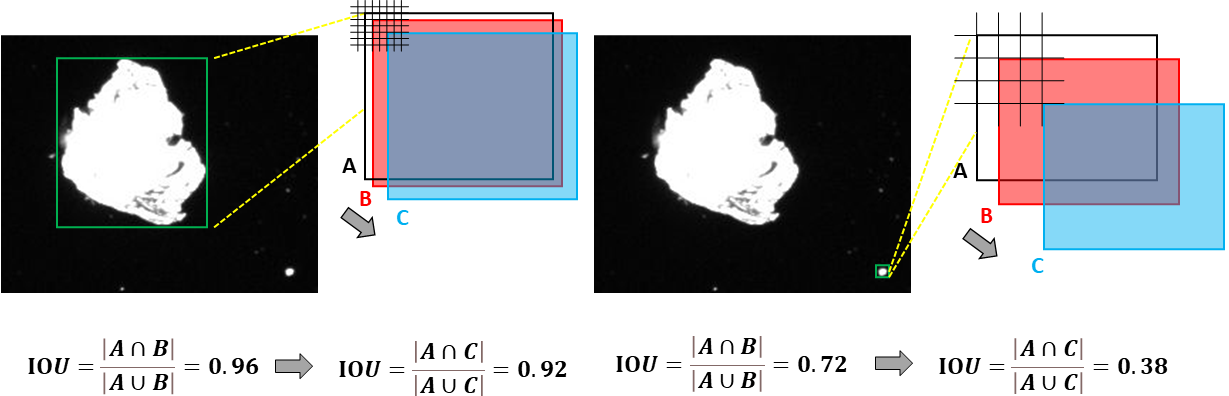
\includegraphics[width=0.5\textwidth]{IOU campare}
    
    \caption {The sensitivity analysis of $IOU$ on small and normal scale objects. Each grid denotes a pixel. box $A$ denotes the ground truth bbox, box $B$, $C$ denote the predicted bbox with 1 pixel and 3 pixels right-down deviation respectively.}

    \label{fig: IOU}
\end{figure}

\subsection{Tiny Head } % 检测头
In the realm of computer vision applications, object detection aims to address the inquiry of "what targets and where are positioned.” In the age of deep learning (DL), a predominant paradigm among modern object detectors involves a backbone for feature extraction and a head dedicated to localization and classification tasks. Under the influence of computational cost, former lightweight detectors invariably employ characteristic maps with low detection resolutions (38 X 38 in SSDLite, 19 × 19 in Pelee, 20 × 20 in ThunderNet). Nonetheless, tiny characteristic maps showing low spatial resolution, can not offer spatially matched characteristics for targets in arbitrary locations, particularly for tiny targets\cite{chen2023tinydet} Such information loss hardly affects large or medium-sized targets. Unfortunately, this is fatal for small objects, as the detector heads struggle to give accurate predictions over highly structured representations, in which the weak signal from small objects is all but eliminated\cite{zhao2022single}. Furthermore, the SISRT-V2 dataset is explored, and it is discovered that it encompasses numerous highly tiny cases,  such as those with bounding boxes of 3 X 3 ~ 5 X 5, which might include no characteristic points through a pervasive characteristic map stride \cite{dai2023one}. Thereby, to handle the difficulty of investigating tiny targets in complex scenes, a new detection head is raised\ref{fig: Head} which consists of a small target detection module. Unlike the conventional detection head that performs classification and regression simultaneously, we decoupled these two tasks into separate branches. Moreover, we added an extra prediction head to the original three-layer detection structure, which is specifically designed for tiny object detection.
% 总结
The performance distinctions in infrared small target detection is largely triggered by two elements. For starters, present label assignment patterns, whether anchor-based or anchor-free, tend to inaccurately mark highly small ground-truth objects as background, which causes the detectors to attach less importance to tiny objects. Secondly, The detection heads designed by conventional object detection methods are difficult to give accurate predictions based on highly structured representations, where small objects fail to detect tiny targets. In conclusion, our conclusions are listed below: 

\begin{itemize}
  \item An effective multi-scale label assignment(MSLA) tactic is introduced. The MSLA can easily displace the point-based label assignment tactics in mainstream detectors and standardized boxes, thereby facilitating their performance on Infrared small targets.       
  \item we designed a multi-scale small target detection head,  and it is capable of improving the detecting performance of tiny objects without losing large targets.
  \item Our experiment results on the SISRT-V2 datasets reached SOTA.
\end{itemize}

% 方法介绍
\section{METHODOLOGY}
The one-stage detection framework ultralytics was selected as our datum line since it is the most convenient and remarkable one-stage detector\cite{glenn_jocher_2022_7347926}. The infrared small targets have a small sample size and few categories, so we add tiny CSDarknet as the backbone. we still keep FPN and PanNet architecture as our head, which is comprised of some bottom-up pathways and some top-down pathways \cite{lin2017feature}\cite{PanNet}. To further optimize the whole architecture, we design an effective Muti-scale label assignment(MSLA) strategy. Then, we designed a multi-scale tiny object detection head to enhance the detecting rate of small targets. While we train the model through the SISRT-V2 dataset by means of a data augmentation tactic (MixUp, Mosaic).
% 插入网络结构图

\begin{figure*}[!t]
    \centering
    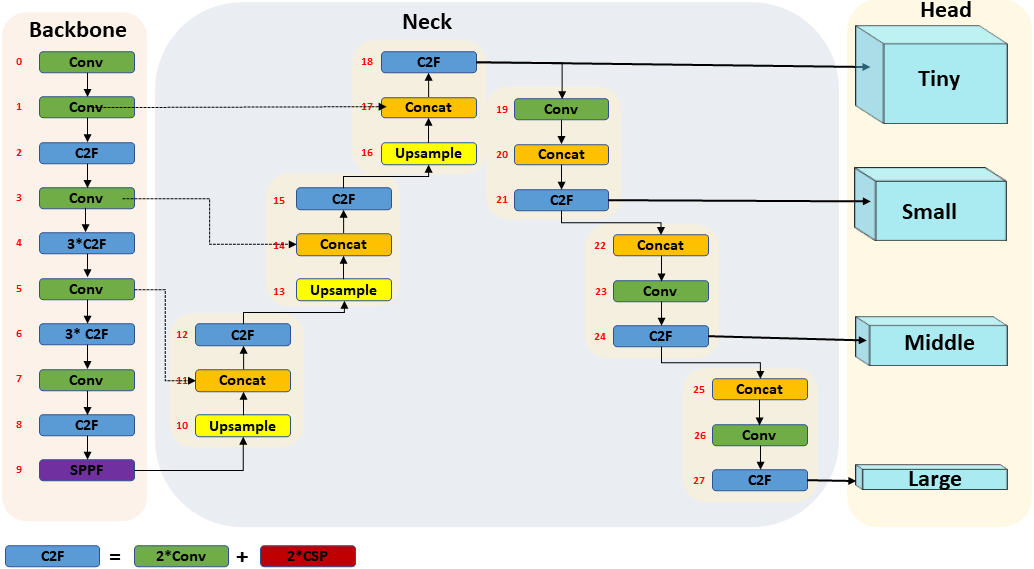
\includegraphics[width=0.8\textwidth]{Net}
    \caption {The architecture of the MSHN. a) CSPDarknet53 backbone with four multi-scale detection heads at the end. b) The Neck uses a structure like PANet.}

    \label{fig: Net}
\end{figure*}

\subsection{MSLA strategy in tiny Object}
Since the most extensive metric is adopted in target detection, IoU has restrictions for assessing the positional correlation between two boundary boxes \cite{xu2021dot}. After continuous improvement, CIOU has been adopted as a mainstream label for assigning losses. However, the enhancements may not address the issue that small targets are vulnerable to IoU. Therefore, for the problem of  tiny and medium-sized infrared objects, we adopt the combination of CIOU and DotD. DotD is introduced as the evaluation index for high-resolution feature images, and for low-resolution images, CIOU is used as the index. This is called the MSLA strategy.

\subsubsection{DIoU}
Distance Intersection over Union(DIoU) considers the overlapping velocity,  distance between the target and the anchor, and scale \cite{zheng2019distanceiou}. The loss function is listed below:
\begin{center} % 居中
\begin{equation}
\mathcal{L}_{D I O U}=1-I O U+\frac{\rho^2\left(\mathbf{b}, \mathbf{b}^{g t}\right)}{C^2}
\end{equation}
\end{center}
where $b$ and $b^{g t}$ represent the center point of the prediction box and the real box. $\rho$ means the Euclidean distance between the center of $b$ and $b^{g t}$, $C$  means diagonal length of the tiniest enclosing box encompassing the two boxes. As it is used in loss function, the regression of the object box is swifter and more steady. 

\subsubsection{CIoU}
considers aspect ratio on the grounds of DIOU metrics\cite{zheng2019distanceiou}. The loss function is defined as below

% 公式插入
\begin{center} % 居中
\begin{equation}
\mathcal{L}_{C I o U}=1-I o U+\frac{\rho^2\left(\mathbf{b}, \mathbf{b}^{g t}\right)}{c^2}+\alpha v
\end{equation}
\end{center}

here ${\alpha}$ represents an active trade-off parameter, 
\begin{center} % 居中
\begin{equation}
\alpha=\frac{v}{(1-I o U)+v}
\end{equation}
\end{center}

$v$ determines the uniformity of aspect ratio
\begin{center} % 居中
\begin{equation}
v=\frac{4}{\pi^2}\left(\arctan \frac{w^{g t}}{h^{g t}}-\arctan \frac{w}{h}\right)^2
\end{equation}
\end{center}
where $w^{g t}$,$h^{g t}$ denote width and height of the bounding box
ground truth, $w$,$h$ denote width and height of boundary box anchor.
\subsubsection{Dot Distance}
Dot Distance (DotD) is derived from the observation that absolute and relative sizes of small boundary boxes are much smaller than those of big or medium-sized boundary boxes. The loss function is as below:

\begin{center} % 居中
\begin{equation}
\mathcal{L}_{D o t D}=1-e^{-\frac{\rho\left(\mathbf{b}, \mathbf{b}^{g t}\right)}{S}}
\end{equation}
\end{center}
$\rho$ denotes the Euclidean distance between the center of  $b$ and $b^{g t}$ as below, and $\mathcal{S}$ is the average size of tiny objects in a certain dataset.

\begin{center} % 居中
\begin{equation}
\mathcal{S}=\sqrt{\frac{\sum_{i=1}^M \sum_{j=1}^{N_i} w_{i j} \times h_{i j}}{\sum_{i=1}^M N_i}}
\end{equation}
\end{center}
Where  $w_ij$ and $h_ij$ denote the width and height of $j$-th bounding box within $i$-th image. $M$ stands for the quantity of images in some dataset, $N_i$ stands for the quantity of the marked boundary boxes within the $i$-th image.


\subsection{Prediction head for tiny objects}
The backbone as a categorization network, can not fulfill the positioning assignment. Furthermore, the head is devised to take responsibility for exploring the position and type of the subject through the characteristics maps from  the  backbone\cite{zhu2021tph}. As shown in \ref{fig: Head}, Integrated with other three predicting heads, our four-head construction can alleviate the passive effect of violent target scale variance. the added predicting head ($a$) originates in an elevated-resolution, low-degree, characteristic map,  which becomes more vulnerable to highly targets. 

\begin{figure}[htbp]
    \centering
    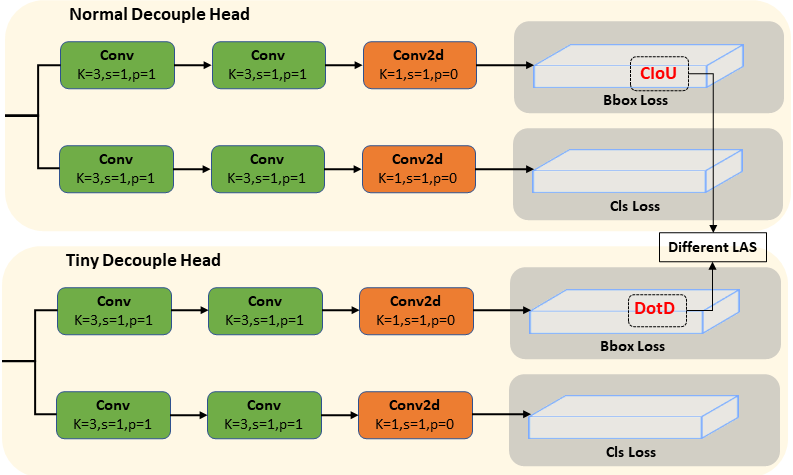
\includegraphics[width=0.4\textwidth]{Head}
    
    \caption {The architecture of Head, contains two main blocks, a normal decouple head block and a tiny decouple head block. Normal decouple head help the network converge better and prevent the network from over fitting. Tiny decouple head can help the current node pay attention to tiny objects.}
    \label{fig: Head}
\end{figure}

% 实验
\section{EXPERIMENTS}
\subsection{Dataset}
SIRST-V2 is a specific dataset, and it is designed for single- frame infrared tiny object detection, where the graphs are chosen from thousands of infrared sequencing for disparate scenes. This dataset involves 1024 typical graphs largely at a resolution of 1280 × 1024. These graphs are acquired from the truthful videos of diverse scenes and they offer a tough trial bed to infrared tiny object detection in intricate real scenes.

\subsection{Experimental Setting}
The total experiments are executed through PyTorch on Ubuntu20 with two RTX 3090. The optimizer is designated as SGD showing a learning velocity of 1e - 2. The target detection is largely assessed by Precision, Recall, and mAP. Target detection outcomes are categorized into TP, FP, FN, along with TN. TP denotes the positive specimen of the accurate categorization; FP denotes the positive specimen of the misclassification; FN denotes the passive specimen of the misclassification; and TN denotes the passive specimen of the accurate categorization. Precision is the proportion of the specimens which are accurately categorized as positive specimens to the whole quantity of detection specimens. The recall is the proportion of specimens of this category which are accurately categorized and recognized to the quantity of specimens in the whole object test sets of this category. In addition, the lost detection rate is used to recognized and assess the algorithm performance for the object frame. The formula is listed as below:

\begin{center} % 居中
\begin{equation}
Re=\frac{TP}{TP + FN}
\end{equation}
\end{center}

\begin{center} % 居中
\begin{equation}
Pr=\frac{TP}{TP + FP}
\end{equation}
\end{center}
We seek to gain the total potential values of Precision and Recall and Precision-Recall curve through calculation. The mean network precision is calculated as the area under the curve. Furthermore, the value varies between 0 and 1


\begin{center} % 居中
\begin{equation}
AP_{IoU}= \int_{0}^{1} P(R) dR
\end{equation}Precision and Recall values and figure out Precision-Recall curve
\end{center}
Precision and Recall values and calculate the Precision-Recall curve
\subsection{Small-target  Detection and Analysis}
To affirm the feasibility and superiority of our proposed model, we compared it with five models on the SIRST-V2 dataset The specific experimental results are presented in Table \ref{tab:univ-compa}. As can be seen in Tables\ref{tab:univ-compa} our model has an AP50 value of 93.1\%, which is significantly better than other detection models. 
\begin{table}[!t]
    \centering
    \caption{Comparison of performance among the proposed algorithm and the other five algorithms in SIRST-V2.}
    \label{tab:univ-compa}
    \begin{tabular}{lcccr}
    \toprule
        \textbf{Method} & $\mathbf{mAP_{50-90}{(\%)}} $ & $ \mathbf{AP_{50}{(\%)}}$ & \textbf{Recall{(\%)}} & \textbf{Precies}  \\ 
        \midrule
        FasterRCNN & 62.28  & 80.7   & 59.2     & 0.68\\ 
        FCOS       & 63.54  & 77.5   & 63.72    & 0.69\\ 
        OSCAR      & 78.8   & 88.8   & 84.43     & 0.83\\
        YOLOV5     & 71.2   & 83.5   & 79.51     & 0.78\\
        YOLOV8     & 82.4   & 91.4   & 90.14       & 0.89\\
        \textbf{Ours} & \textbf{83.9} & \textbf{93.1}   &  \textbf{94.0}    &  \textbf{93.0} \\
    \bottomrule
    \end{tabular}
\end{table}

\begin{figure}[!t]
    \centering
    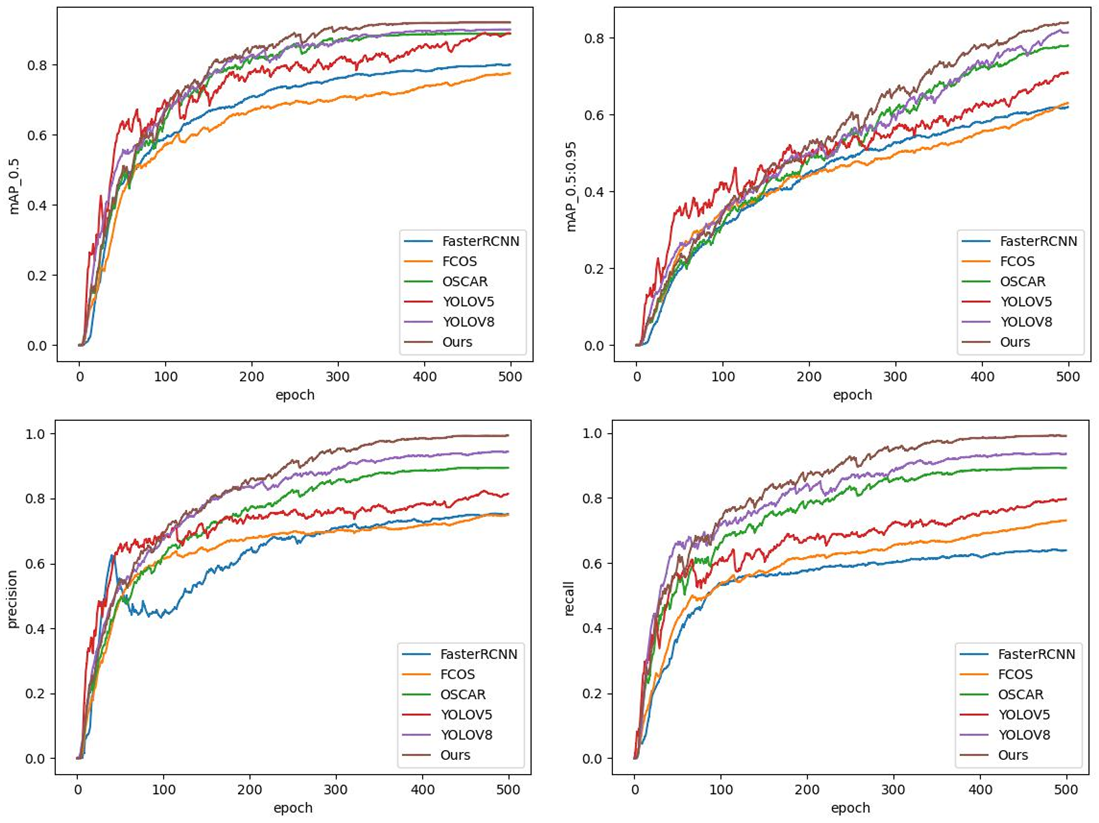
\includegraphics[width=8cm]{graph}
    \caption {Comparison of training results among the proposed algorithm and the other five algorithms in SIRST-V2.}

    \label{fig: graph}
\end{figure}
\begin{center}
\begin{figure*}[!t]
    \centering
    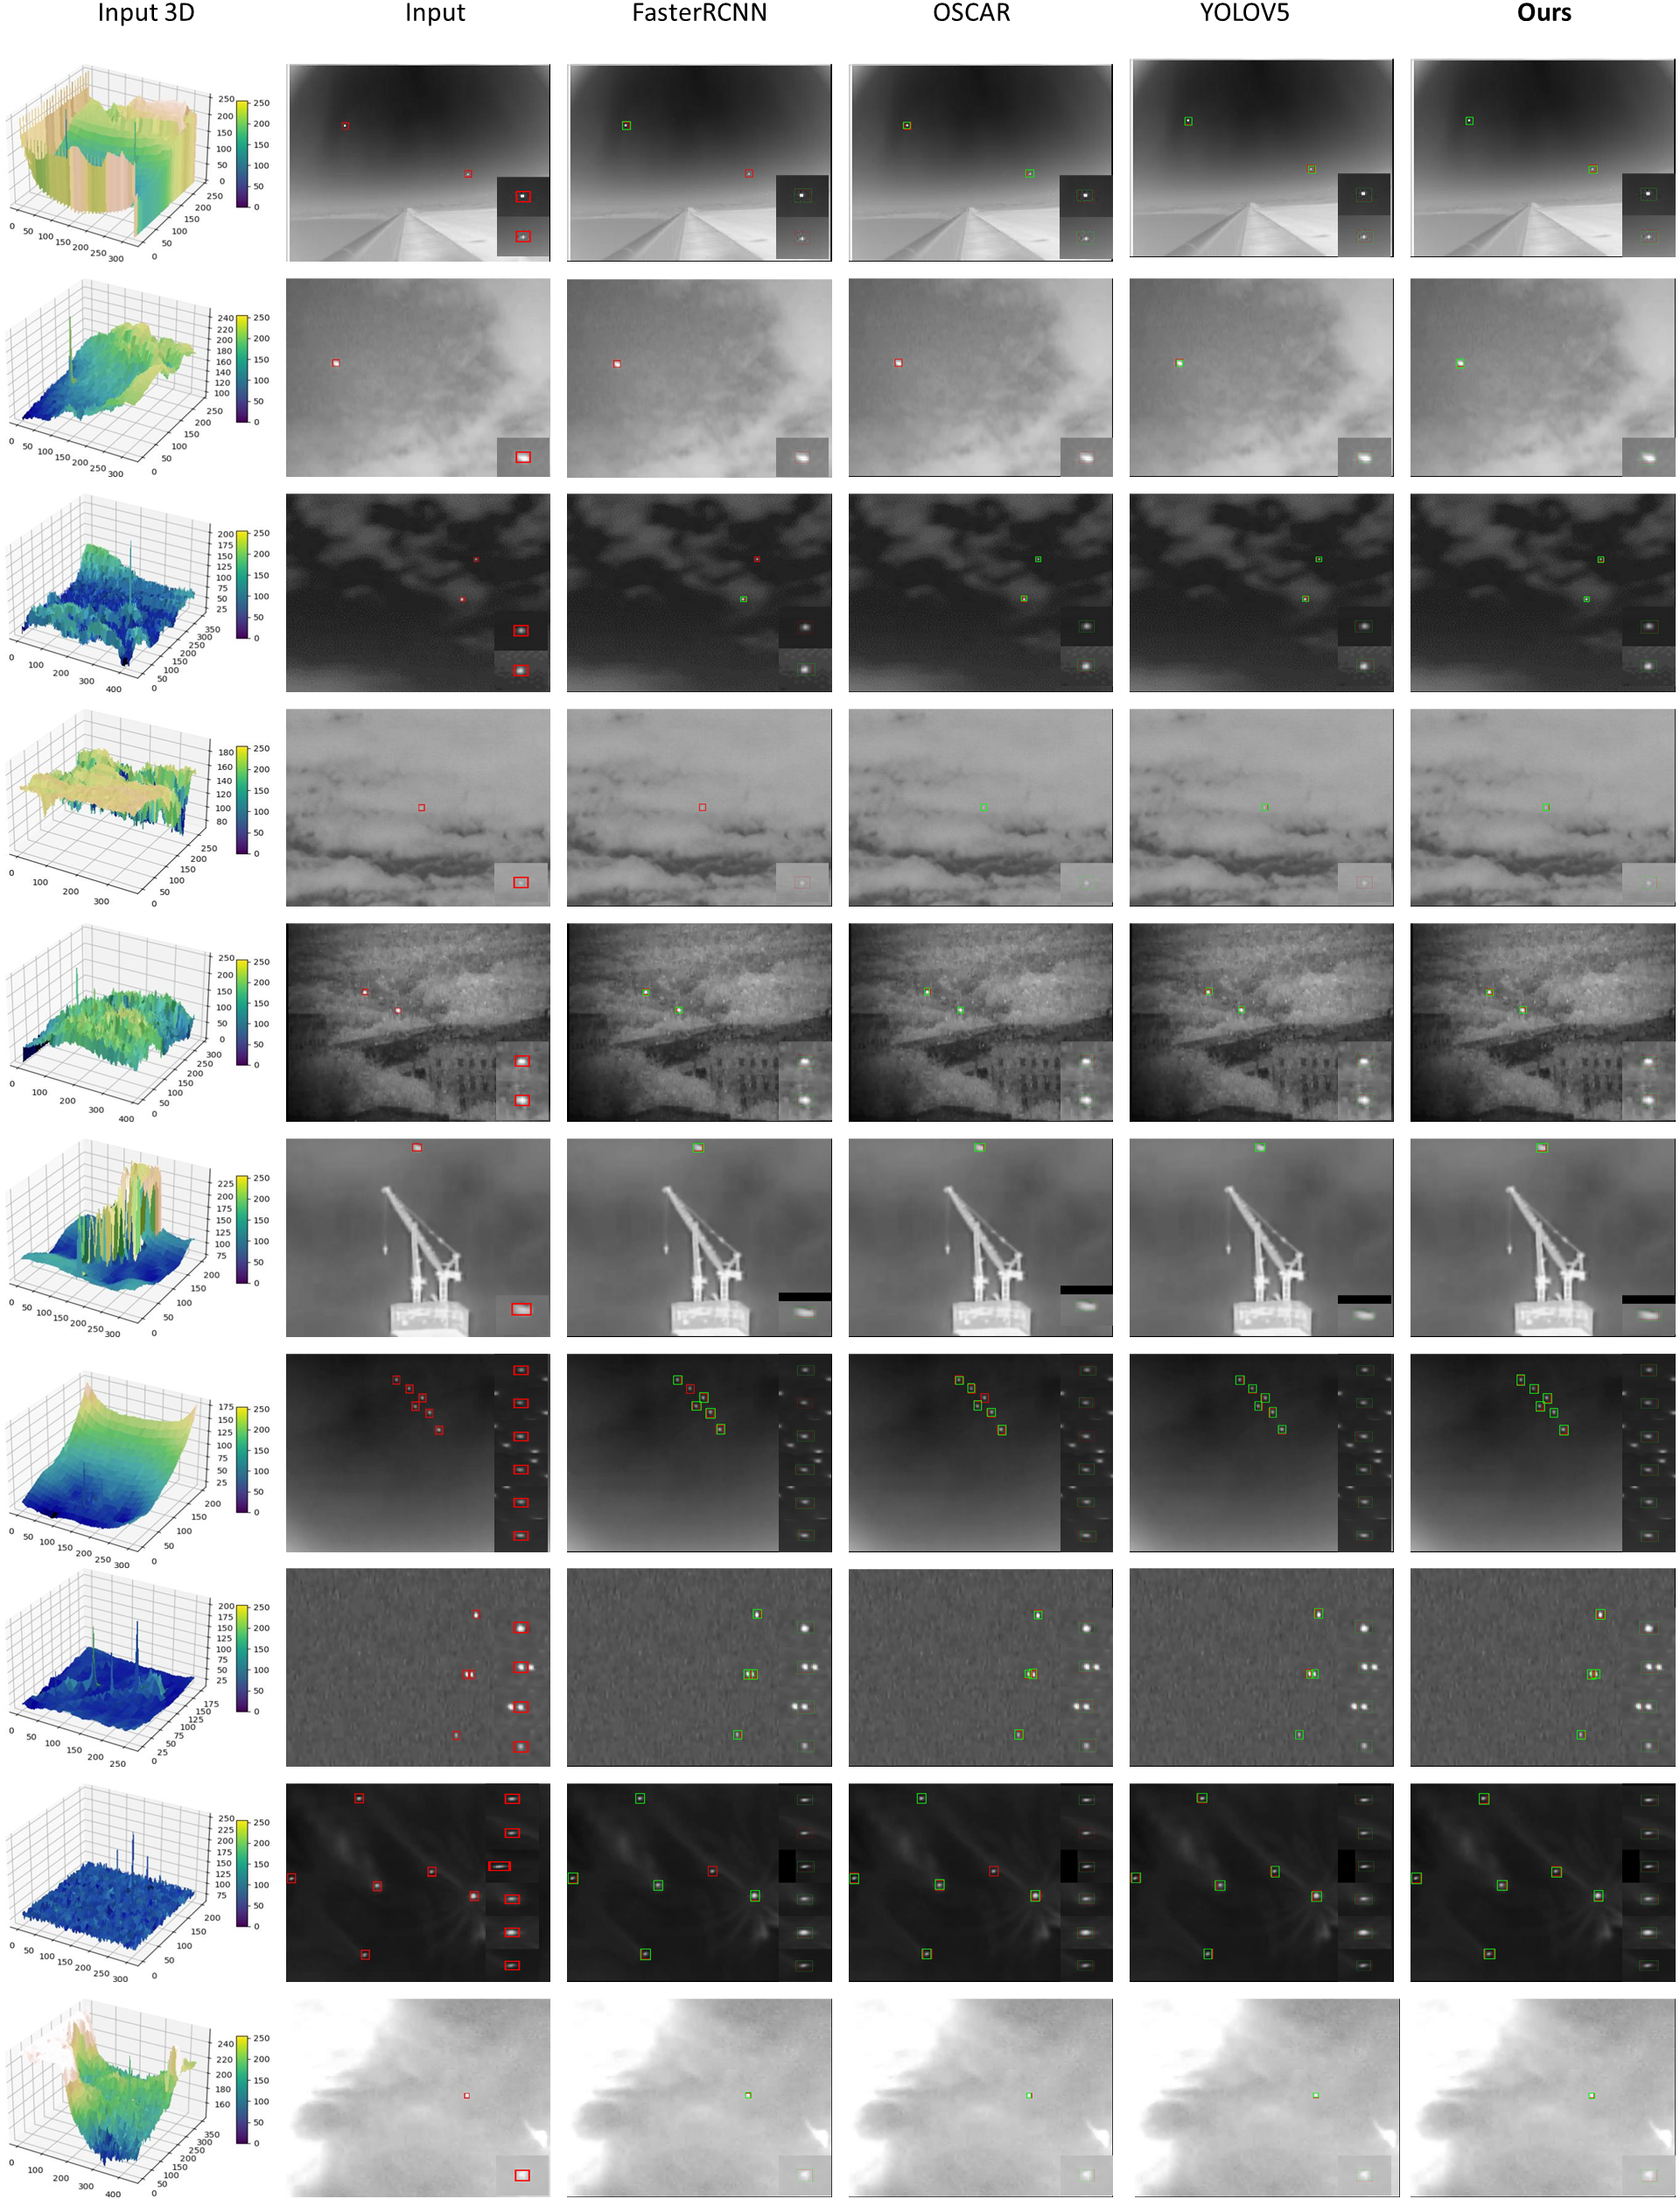
\includegraphics[width=0.7\textwidth]{experience}
    \caption {Comparison of visualization results on SIRST-V2 dataset.}

    \label{fig: experience}
\end{figure*}
\end{center}

% 结论
\section{Conclusion}
we introduce a effective Muti-scale label assign- ment(MSLA)  tactic.  The  MSLA  easily displace the standard box and point-based label task tactics in mainstream detectors. Hence, their performance on Infrared small target are facilitated. Our designed a multi-scale small target detection head, which can enhance the detecting performance of tiny objects without losing large targets. Widespread tests and analyses on SIRST-V2 dataset deeply verify the efficiency of MLSA-YOLOV8. 


\ifCLASSOPTIONcaptionsoff
  \newpage
\fi

% 打印引用
\printbibliography

\end{document}

